\chapter{Cinematica dei Robot}

In questo capitolo studieremo il metodo geometrico per ottenere la posizione dell'end-effector a partire dalle joint variables (angoli o posizioni). Notare che qua non consideriamo forze e coppie.
\vspace*{5pt}
\begin{figure}[H]
	\centering
	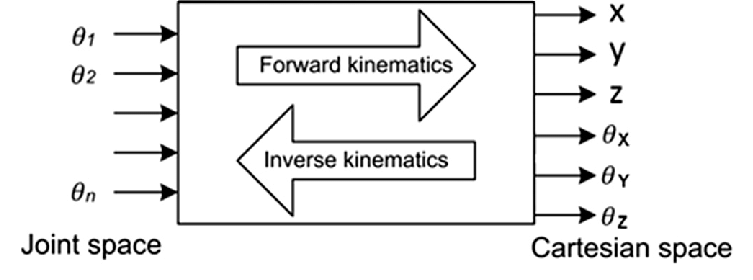
\includegraphics[width=0.5\linewidth]{images/kinematics_1}
	\label{fig:kinematics1}
\end{figure}


\section{Cinematica Diretta}

Sia $\mathcal{R}_b$ il \textbf{base frame} solidale con la base del robot, e sia $\mathcal{R}_e$ un sistema di riferimento mobile solidale con la punta operativa (end-effector) del robot.
Di conseguenza, la posa dell'end-effector sarà data dalla posizione ed orientamento di $\mathcal{R}_e$ rispetto a $\mathcal{R}_b$.

La cinematica diretta ha come scopo il calcolo della posa della punta operativa in funzione delle variabili giunto $q_i$, quindi dobbiamo esprimere la relazione fra i 2 RF in modo analitico.
Possiamo osservare che $\mathcal{R}_e$ può essere può essere rappresentato nel base frame $\mathcal{R}_b$ per mezzo della matrice di trasformazione:
$$
{}^b\textbf{T}_e(\mathbf{q}) = 
\begin{bmatrix}
	{}^b\mathbf{R}_e(\mathbf{q}) & {}^b\textbf{p}_e(\mathbf{q}) \\
	\mathbf{0} & 1
\end{bmatrix}
=
\begin{bmatrix}
	{}^b\mathbf{n}_e(\mathbf{q}) &
	{}^b\mathbf{s}_e(\mathbf{q}) & 
	{}^b\mathbf{a	}_e(\mathbf{q}) & 
	{}^b\textbf{t}_e(\mathbf{q}) \\
	0 & 0 & 0 & 1
\end{bmatrix}
$$
dove:
\begin{itemize}
	\item ${}^b\textbf{p}_e(\mathbf{q})$ è l'origine di $\mathcal{R}_e$ in $\mathcal{R}_b$
	\item ${}^b\mathbf{R}_e(\mathbf{q})$ è la matrice di rotazione di $\mathcal{R}_e$ rispetto a $\mathcal{R}_b$
	\item $	{}^b\mathbf{n}_e(\mathbf{q}), {}^b\mathbf{s}_e(\mathbf{q}), {}^b\mathbf{a	}_e(\mathbf{q})$ sono i 3 versori del sistema di riferimento dell'end-effector $\mathcal{R}_e$ (rispettivamente \textbf{approach}, \textbf{sliding} e \textbf{normal}).
\end{itemize}

Il nome dei 3 versori deriva dal fatto che:
\begin{itemize}
	\item approach: posizionato nella direzione di approccio dell’utensile al pezzo
	\item sliding: posizionato nel piano di scorrimento (sliding) delle ganasce
	\item normal: ottenuto come prodotto vettoriale fra i primi due (e quindi normale a loro).
\end{itemize}

\begin{figure}[H]
	\begin{subfigure}{0.65\linewidth}
		\centering
		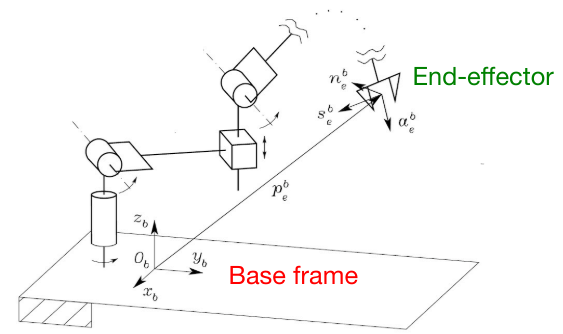
\includegraphics[width=0.9\linewidth]{images/kinematics_2}
		\caption{Esempio}
		\label{fig:kinematics2}
	\end{subfigure}
	\begin{subfigure}{0.3\linewidth}
		\centering
		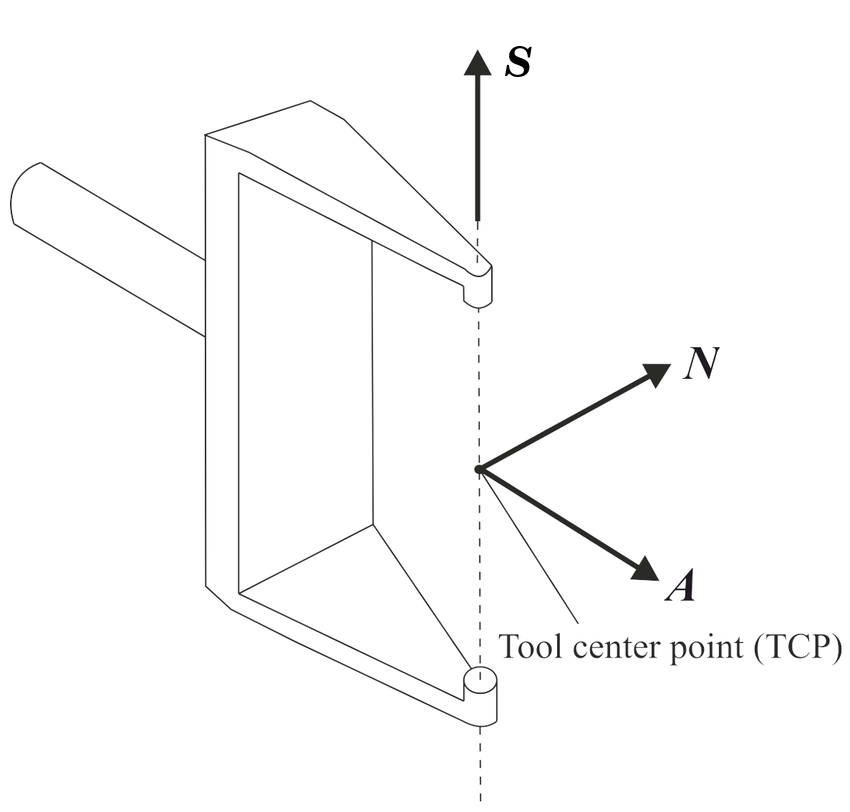
\includegraphics[width=1\linewidth]{images/kinematics_3}
		\caption{Versori di $\mathcal{R}_e$}
		\label{fig:kinematics3}
	\end{subfigure}
\end{figure}


Visto che
$$
\mathbf{x} = (x, y, z, \phi, \theta, \psi) = {}^b\textbf{T}_e(\mathbf{q})
$$
risolvere la cinematica diretta significa determinare trovare la matrice $\mathbf{T}$, che è specifica per ogni particolare robot (essendo dipendente dalla sua struttura fisica).


Soltanto nel caso di manipolatori estremamente semplici, con pochi gradi di libertà, è possibile risolvere il problema della cinematica diretta delle posizioni per via geometrica (i.e a manina). In generale, per un manipolatore con $n + 1$ links, collegati da $n$ giunti, è necessario ricorrere ad una procedura sistematica, basata su:
\begin{itemize}
	\item Definizione di $n + 1$ sistemi di riferimento $\mathcal{R}_0 \dots \mathcal{R}_n$ ciascuno solidale con un braccio del robot dalla base (braccio/link 0, $\mathcal{R}_0 \equiv \mathcal{R}_b$) fino all’ultimo braccio (n)
	\item Calcolo della matrice di trasformazione come prodotto (composizione) delle varie matrici di trasformazione fra i singoli sistemi di riferimento: 
	$$
	{}^b\textbf{T}_e(\mathbf{q}) \equiv {}^0\textbf{T}_n(\mathbf{q}) = 
	{}^b\textbf{T}_1(q_1)
	{}^1\textbf{T}_2(q_2)
	\cdots
	{}^{n-1}\textbf{T}_n(q_n)
	$$
\end{itemize}

\begin{figure}[H]
	\centering
	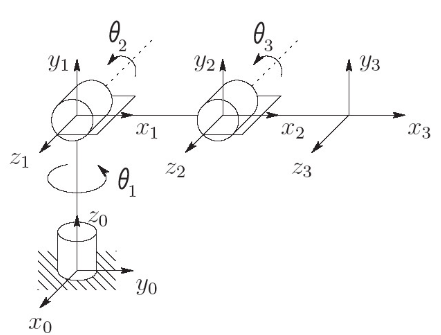
\includegraphics[width=0.5\linewidth]{images/kinematics_4}
	\caption{Sistemi di riferimento $\mathcal{R}_0 \dots \mathcal{R}_n$}
	\label{fig:kinematics4}
\end{figure}

Nota: la matrice $\mathbf{T(q)}$ \underline{non} è costante, ma dipende dalla configurazione corrente del robot!

Inoltre, se per qualche motivo la base e l'end effector non coincidono con i frame $0$ e $n$ ci basta aggiungere le 2 rispettive trasformazioni
$$
{}^b\textbf{T}_e(\mathbf{q}) =
{}^b\textbf{T}_0
{}^0\textbf{T}_n(\mathbf{q})
{}^n\textbf{T}_e
$$
che in generale sono costanti e non dipendono da $\mathbf{q}$.


\section{Convenzioni di Denavit-Hartenberg}
Queste convenzioni stabiliscono delle regole generali e sistematiche per la definizione dei sistemi di riferimento di ogni link. In particolare ci permettono di definire in maniera sistematica la matrice ${}^{i-1}\textbf{T}_i(q_i)$.

Se seguiamo le regole della convenzione (per il posizionamento dei RF), ogni matrice di quel tipo sarà funzione di soli 4 parametri:
\begin{itemize}
	\item $a_i$: lunghezza del link $i$
	\item $\alpha_i$: twist del link $i$
	\item $d_i$: offset del link $i$
	\item $\theta_i$: angolo del giunto $i$
\end{itemize}
Inoltre, visto che la matrice finale ${}^{i-1}\textbf{T}_i(q_i)$ è dipendente solo da una variabile ($q_i$), solo 1 fra quei 4 parametri potrà essere variabile, mentre gli altri saranno costanti. In particolare quelli variabili sono:
\begin{itemize}
	\item Se giunto rotoidale: $\theta_i = q_i$
	\item Se giunto prismatico: $d_i = q_i$
\end{itemize}


\subsection{Sistemi di riferimento}

\begin{figure}[b]
	\centering
	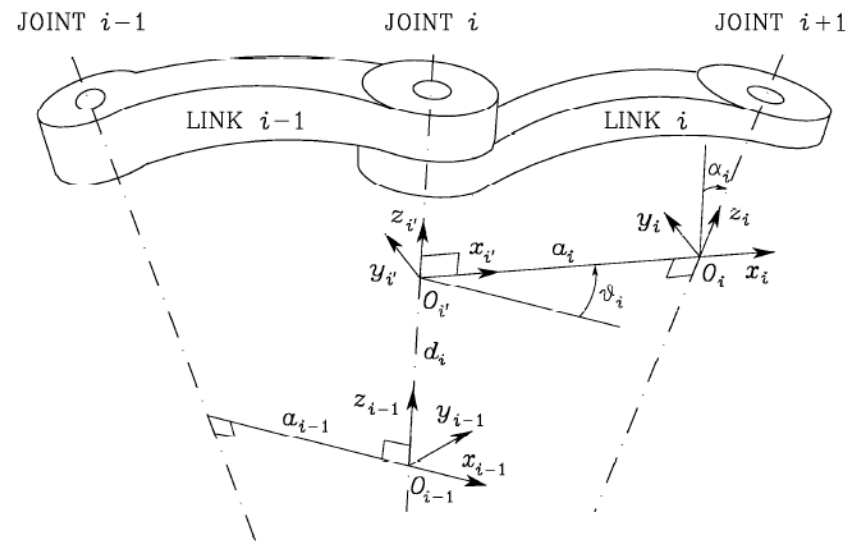
\includegraphics[width=0.6\linewidth]{images/kinematics_5}
	\caption{Convenzione di Denavit-Hartenberg}
	\label{fig:kinematics5}
\end{figure}

Introduciamo ora il metodo che dovremmo utilizzare per definire i vari RF. \\
In particolare vanno definiti $n + 1$ sistemi di riferimento $\mathcal{R}_i$, ognuno solidale con uno specifico braccio/link $i$ (importante notare che questo RF quindi si muoverà con quel particolare braccio, che a sua volta è attuato dal joint $i$)

Un ulteriore sistema di riferimento solidale con la punta operativa può essere introdotto, orientandone gli assi in maniera consona alla definizione del compito da svolgere.

\vspace*{25pt}
\textbf{Il sistema di riferimento $\mathcal{R}_i$ solidale con $\textit{LINK}_i$ viene definito secondo le seguenti regole\footnote{Notazioni slide italiano: $b_i \equiv \textit{LINK}_i \, \ g_i \equiv \textit{JOINT}_i$}:}\\

\circled{1} \textbf{Asse $z_i$ e origine $O_i$}
\begin{itemize}
	\item \textbf{L’asse} $\boldsymbol{z_i}$ è posto lungo l’asse di movimento di $g_{i+1}$ (asse di rotazione o di traslazione a seconda del tipo di giunto)
	\item \textbf{L’origine} $\boldsymbol{O_i}$ è posta all’intersezione di $z_i$ con la normale comune (\textit{common normal}) fra gli assi $z_{i-1}$ e $z_i$.
	La normale comune è quella retta perpendicolare ad entrambi gli assi (nota entrambi angoli retti nella figura)
	\item \textbf{Casi particolari}:
	\begin{itemize}
		\item $\boldsymbol{\mathcal{R}_0}$: qua è univocamente definita solo la direzione di $z_0$, data dall’asse di movimento di $g_1$; l’origine $O_0$ e $x_0$ possono essere fissati a piacimento
		\item $\boldsymbol{\mathcal{R}_n}$: visto che non esiste il giunto $g_{n+1}$, $z_n$ e $O_n$ non sono univocamente definiti. Per consuetudine si fissa l’origine nel centro della pinza. E visto che tipicamente l'ultimo giunto è rotoidale, $z_n$ è presa coincidente a a $z_{n-1}$ (così da semplificare la matrice di rotazione, visto che otterremo elementi nulli)
	\end{itemize}
\end{itemize}

\begin{figure}[H]
	\centering
	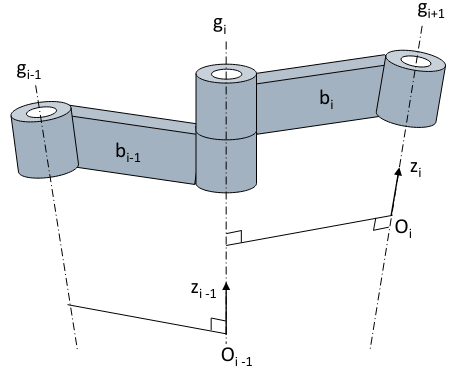
\includegraphics[width=0.4\linewidth]{images/kinematics_6}
	\caption{Assi $z$ e origini}
	\label{fig:kinematics6}
\end{figure}



\circled{2} \textbf{Asse $x_i$ e $y_i$}
\begin{itemize}
	\item \textbf{L’asse $\boldsymbol{x_i}$} è fissato lungo la normale comune fra gli assi $z_{i-1}$ e $z_i$
	\begin{itemize}
		\item Se $z_{i-1}$ e $z_i$ si intersecano, l’origine di $\mathcal{R}_i$ coincide con il loro punto di intersezione e la direzione di $x_i$ (ortogonale a $z_i$) è arbitraria
		\item se $z_{i-1}$ e $z_i$ sono paralleli, l’origine può essere posta in un punto a scelta e $x_i$ appartiene al piano normale a $z_{i-1}$ e $z_i$ con direzione e verso arbitrari 
	\end{itemize}
	\item \textbf{L’asse $\boldsymbol{y_i}$} completa la terna destrorsa
\end{itemize}


\begin{figure}[H]
	\centering
	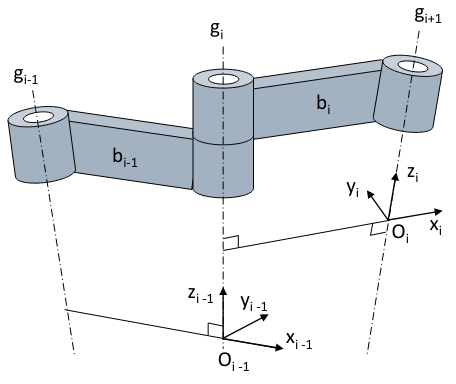
\includegraphics[width=0.4\linewidth]{images/kinematics_7}
	\caption{Assi $x$ e $y$}
	\label{fig:kinematics7}
\end{figure}



\circled{3} \textbf{Parametri di DH}\\
Per comprendere meglio i parametri di DH possiamo introdurre un sistema di riferimento "intermedio" $\mathcal{R}_{i'}$ (vedi fig. \ref{fig:kinematics9}):
\begin{itemize}
	\item $z_{i'}$ diretto lungo $z_{i-1}$
	\item $O_{i'}$ posta all’intersezione di $z_{i-1}$ con la normale comune fra $z_{i-1}$ e $z_i$
	\item $x_{i'}$ diretto lungo la normale comune fra	$z_{i-1}$ e $z_i$ (come $x_i$)
\end{itemize}

\setlength{\fboxsep}{7pt} % Adjust the padding as needed
\fbox{
	\begin{minipage}{\textwidth}
		La posizione e l’orientamento di $\mathcal{R}_i$ sono completamente specificati rispetto a $\mathcal{R}_{i-1}$ dai seguenti 4 parametri:
		\begin{itemize}
			\item $\boldsymbol{d_i} \rightarrow$ \textbf{link offset}: coordinata di $O_{i'}$ lungo $z_{i-1}$
			\item $\boldsymbol{\theta_i} \rightarrow$ \textbf{joint angle}: angolo di rotazione da $x_{i-1}$ a $x_i$ attorno all'asse $z_{i'}$ (positivo quando la rotazione è anti-oraria)
			\item $\boldsymbol{a_i} \rightarrow$ \textbf{link length}: distanza (con segno) fra $O_i$ e $O_{i'}$
			\item $\boldsymbol{\alpha_i} \rightarrow$ \textbf{link twist}: angolo di rotazione da $z_{i-1}$ a $z_i$ attorno all'asse $x_i$ (positivo quando la rotazione è anti-oraria)
		\end{itemize}
	\end{minipage}
}

\begin{figure}[H]
	\begin{subfigure}{0.5\linewidth}
		\centering
		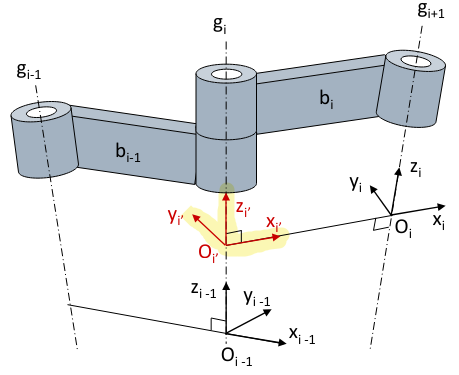
\includegraphics[width=0.95\linewidth]{images/kinematics_8}
		\caption{RF intermedio}
		\label{fig:kinematics8}
	\end{subfigure}
	\hfill
	\begin{subfigure}{0.5\linewidth}
		\centering
		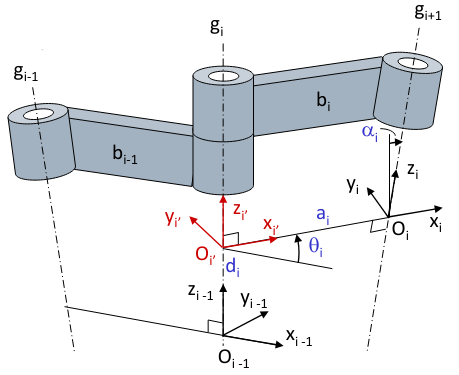
\includegraphics[width=0.95\linewidth]{images/kinematics_9}
		\caption{Parametri di DH}
		\label{fig:kinematics9}
	\end{subfigure}
	\caption{}
\end{figure}





\subsection{Trasformazione delle coordinate}
Ora, come possiamo usare questi parametri per ottenere $\mathbf{T(q)}$?\\


\circled{1} \boldmath$\mathcal{R}_{i-1} \rightarrow \mathcal{R}_{i'}$\unboldmath

$\mathcal{R}_{i'}$ (partendo da $\mathcal{R}_{i-1}$) è dato da una translazione $d_i$ lungo $z_{i-1}$ seguito da una rotazione di $\theta_i$ attorno a $z_i$, quindi:
$$
{}^{i-1}\mathbf{T}_{i'}
=
\begin{bmatrix}
	c\theta_i & -s\theta_i & 0 & 0 \\
	s\theta_i & c\theta_i & 0 & 0 \\
	0 & 0 & 1 & d_i \\
	0 & 0 & 0 & 1
\end{bmatrix}
$$


\vspace*{5pt}
\circled{2} \boldmath$\mathcal{R}_{i'} \rightarrow \mathcal{R}_{i}$\unboldmath

$\mathcal{R}_{i}$ (partendo da $\mathcal{R}_{i'}$) è dato da una translazione $a_i$ lungo $x_{i'}$ seguito da una rotazione di $\alpha_i$ attorno a $x_i$, quindi:
$$
{}^{i'}\mathbf{T}_{i}
=
\begin{bmatrix}
	1 & 0 & 0 & a_i \\
	0 & c\alpha_i & -s\alpha_i & 0 \\
	0 & s\alpha_i & c\alpha_i & 0 \\
	0 & 0 & 0 & 1
\end{bmatrix}
$$



\vspace*{5pt}
\circled{3} \boldmath$\mathcal{R}_{i-1} \rightarrow \mathcal{R}_{i}$\unboldmath

Infine, componendo le due trasformazioni, otteniamo:
$$
{}^{i-1}\mathbf{T}_{i}(q_i)
=
{}^{i-1}\mathbf{T}_{i'}
{}^{i'}\mathbf{T}_{i}
=
\begin{bmatrix}
	c\theta_i & -s\theta_ic\alpha_i & s\theta_is\alpha_i & a_ic\theta_i \\
	s\theta_i & c\theta_ic\alpha_i & -c\theta_is\alpha_i & a_is\theta_i \\
	0 & s\alpha_i & c\alpha_i & d_i \\
	0 & 0 & 0 & 1
\end{bmatrix}
$$

Quindi, per ottenere ${}^0\mathbf{T}_{n}(\mathbf{q})$ non ci basterà che comporre le varie matrici ottenute sopra, le quali possono essere facilmente ricavate inserendo i giusti valori dei 4 parametri.





\section{Operational space e Joint space}

L'\textbf{operational space (task space, o cartesian space)} è quello spazio dove è definito il vettore di posizioni e orientamento dell'end effector, ovvero:
$$
\boldsymbol{x}_e = (\boldsymbol{p}_e, \boldsymbol{\phi}_e) = (x, y, z, \phi, \theta, \psi)
$$

In contrasto, il \textbf{joint space (o configuration space)} è quello spazio dove è definito:
$$
\mathbf{q} = [q_1 \dots q_n] \in \mathbb{R}^n
$$
$q_i$ è la singola variabile di un giunto (ricordiamo che a ciascun giunto corrisponde un grado di libertà). In particolare:
\begin{itemize}
	\item Giunto rotoidale: $q_i = \theta_i$ (rotazione)
	\item Giunto prismatico: $q_i = d_i$ (traslazione)
\end{itemize}

La postura della catena cinematica è quindi determinata dalla posa di tutti i corpi rigidi (i bracci) che la costituiscono ed è una funzione di $\mathbf{q}$:
$$
\boldsymbol{x}_e 
= 
\begin{bmatrix}
	x(q_1, \dots, q_n) \\
	y(q_1, \dots, q_n) \\
	z(q_1, \dots, q_n) \\
	\phi(q_1, \dots, q_n) \\
	\theta(q_1, \dots, q_n) \\
	\psi(q_1, \dots, q_n) \\
\end{bmatrix}
= 
\boldsymbol{k}(\boldsymbol{q})
$$
dove $\boldsymbol{k}(\boldsymbol{q})$ è la \textbf{funzione di cinematica diretta}.

\textbf{Una soluzione} di questa funzione è data dalla matrice ${}^0\mathbf{T}_{n}(\mathbf{q})$ definita prima. Notiamo che però la soluzione trovata utilizza una rappresentazione non minimale dell'assetto (matrice di rotazione), mentre nella definizione di $k(q)$ è minimale (angoli di eulero).

\begin{figure}[!ht]
	\centering
	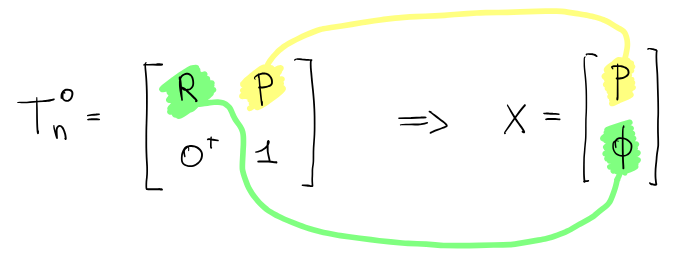
\includegraphics[width=0.6\linewidth]{images/kinematics_10}
	\caption{}
	\label{fig:kinematics10}
\end{figure}




\section{Workspace (spazio di lavoro)}
Con riferimento allo spazio operazionale lo \textbf{spazio di lavoro} del robot è definito da tutti quei punti di $\boldsymbol{x}_e$ ottenuti eseguendo tutte le possibili configurazioni dei giunti.
\begin{figure}[!bh]
	\centering
	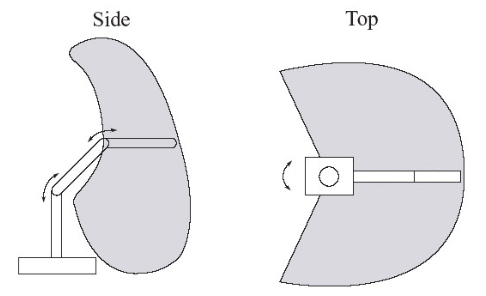
\includegraphics[width=0.5\linewidth]{images/kinematics_11}
	\caption{Esempio di spazio di lavoro}
	\label{fig:kinematics11}
\end{figure}

All'interno di questo spazio possiamo specificarne due:
\begin{itemize}
	\item \textbf{Reachable workspace}: è lo spazio di lavoro che l'end-effector può raggiungere con \underline{almeno un} orientamento
	\item \textbf{Dexterous workspace}: è lo spazio di lavoro che l'end-effector può raggiungere con \underline{più di un} orientamento. Ovviamente $\textit{dexterous workspace} \subset \textit{reachable workspace}$
\end{itemize}

Ad esempio, la punta di un manipolatore con meno di 6 gradi di libertà non può certamente raggiungere qualunque posa nello spazio 3D.





\section{Accuracy e Repeatability}

Per via di imprecisioni meccaniche, esisteranno sempre delle discrepanze fra i parametri DH nominali e quelli reali. Questa discrepanza prende il nome di \textbf{accuratezza}. Un requisito necessario per averla elevata è avere una struttura \textbf{rigida}.\\
Nei manipolatori moderni è $< 1$mm e solitamente varia con la posizione dell'end-effector.

La \textbf{repetibilità} invece è la capacità del manipolatore di ritornare ad una posizione precedente con un certo grado di precisione (questa dipende dalla struttura meccanica ma anche dalle strategie di controllo utilizzate e dalla precisione dei trasduttori).

\begin{figure}[!hb]
	\centering
	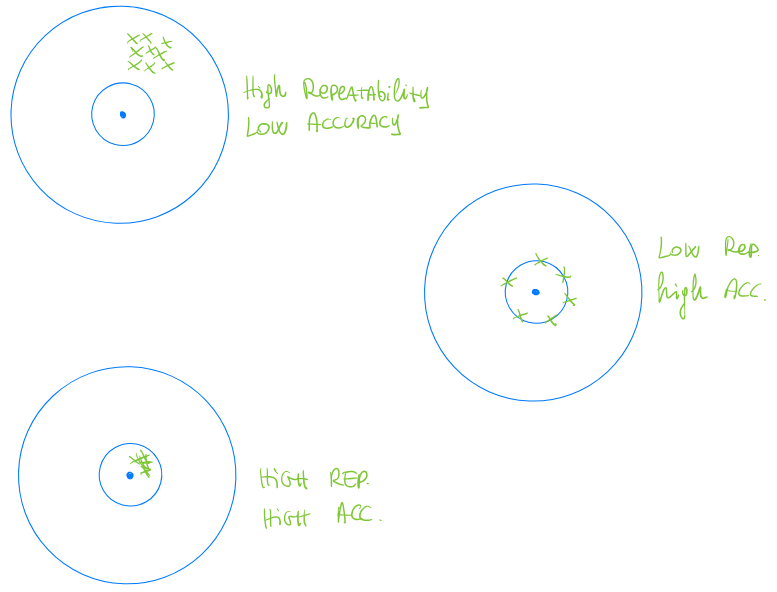
\includegraphics[width=0.6\linewidth]{images/kinematics_15}
	\caption{Esempi accuracy e repeatability}
	\label{fig:kinematics15}
\end{figure}




\section{Cinematica inversa}
Il problema della cinematica inversa delle posizioni consiste nella determinazione delle variabili giunto $\boldsymbol{q}$ corrispondenti ad un dato $\boldsymbol{x}_e$ o una data ${}^b\mathbf{T}_{e}(\mathbf{q})$.

L’esistenza della soluzione a tale problema è garantita solo se la posizione e l’orientamento della punta appartengono allo spazio di lavoro (di destrezza) del manipolatore.

Il \textbf{problema} della cinematica inversa delle posizioni è \textbf{molto più complesso} di quello della cinematica diretta: 
\begin{itemize}
	\item Le \textbf{equazioni} da risolvere sono in generale \textbf{non lineari} (a causa di $sin$, $cos$, ...) e di conseguenza non è sempre possibile trovare una soluzione in forma chiusa
	\item \textbf{Possono esistere molteplici soluzioni} (cioè più posture del manipolatore corrispondenti alla stessa posizione ed assetto della punta). Addirittura possono risultare infinite nel caso di un manipolatore ridondante
	\item \textbf{Possono anche non esistere proprio soluzioni}: vincoli cinematici nella struttura reale del robot potrebbero ridurre o azzerare il numero di soluzioni "ammissibili"
\end{itemize}

Putroppo \textbf{non esistono procedure} per il calcolo della cinematica inversa di un robot: la determinazione della soluzione in forma chiusa è fortemente basata su \textbf{intuizioni algebriche e geometriche}.\\
Nei casi in cui sia impossibile (o estremamente difficoltoso) giungere alla soluzione in forma chiusa si ricorre a \textbf{tecniche numeriche di soluzione}, ad esempio:
$$
\min_{q} = \| \boldsymbol{x}_{\text{e ref}} - \boldsymbol{k}(\boldsymbol{q}) \|
$$

Per quanto riguarda quest'ultime abbiamo come vantaggio che sono applicabili a qualunque struttura cinematica, ma che però non forniscono (in generale) tutte le possibili soluzioni.\\
Alternativamente è possibile utilizzare la \textbf{Jacobiana} (che vedremo più avanti), invertendo le velocità ed integrando per ottenere la posizione.



\subsection{Manipolatore con polso sferico}

Nel caso di un manipolatore a 6 DOF con polso sferico, \textbf{è possibile disaccoppiare} il problema della cinematica inversa in due sottoproblemi, relativi uno alla determinazione della posizione (del polso) e l’altro dell’assetto (dell'end-effector).\\
Indichiamo il centro del polso (inteso come la posizione in cui si intersecano gli assi dei suoi giunti) con $\boldsymbol{W}$.
\vspace*{-3pt}
\begin{figure}[H]
	\centering
	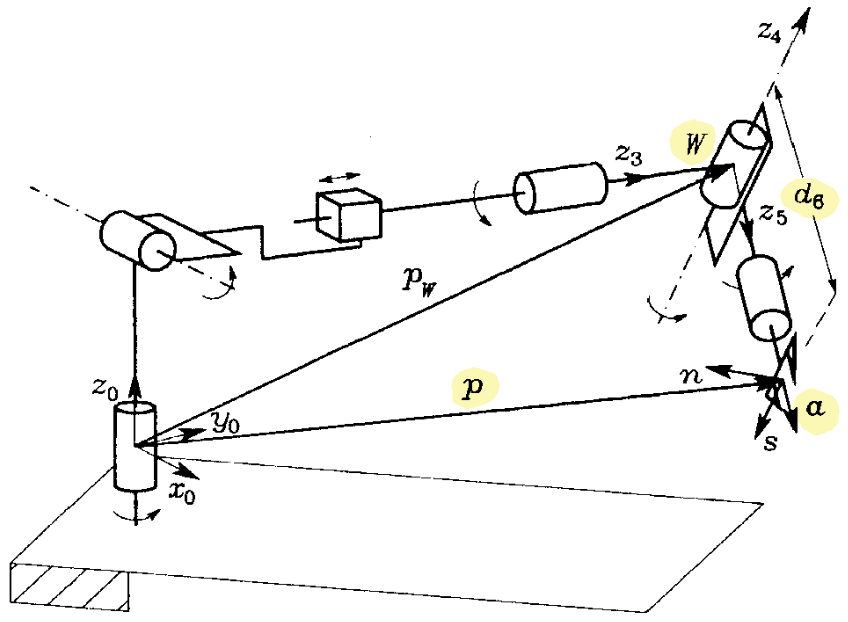
\includegraphics[width=0.5\linewidth]{images/kinematics_16}
	\label{fig:kinematics16}
\end{figure}

Se $\boldsymbol{p}$ e $\boldsymbol{(n,s,a)}$ (posizione e orientamento del polso) sono noti:
$$
\boldsymbol{W} = \boldsymbol{p} - d_6 \boldsymbol{a}
$$
poichè $W$, rappresentato dal vettore $p_W$, è ottenibile come sottrazione vettoriale fra $p$ e il vettore lungo $d_6$ orientato nel verso di $a$.

Grazie a questa osservazione, possiamo ora suddividere il problema della cinematica inversa in 2 parti:
\begin{enumerate}
	\item Dalla posizione $\boldsymbol{p}$ della punta è possibile ricavare $\boldsymbol{W}$ e quindi risolvere la cinematica inversa per determinare le tre variabili giunto "della spalla": calcola la posizione del polso $\boldsymbol{W}(q_1, q_2, q_3)$ tramite la formula sopra, e poi risolvi la cinematica inversa per $(q_1, q_2, q_3)$
	\item Tenendo conto della cinematica ormai nota della spalla, si passa al calcolo dei restanti $q_i$ a partire dall’assetto della punta: calcola ${}^0R_3(q_1, q_2, q_3) \implies {}^3R_6(\theta_1, \theta_2, \theta_3) = ({}^0R_3)^T \ {}^0	R_e$ e quindi risolvi la cinematica inversa per $(\theta_1, \theta_2, \theta_3)$ tramite ${}^3R_6$
\end{enumerate}